
\tikzstyle{block} = [fill=red!20, draw,rectangle,  text centered, rounded corners, minimum height=2em]
\tikzstyle{block2} = [fill=blue!20,draw,rectangle,  text centered, rounded corners, minimum height=2.5em]
\tikzstyle{block3} = [fill=green!20,draw,rectangle,  text centered, rounded corners, minimum height=2em]
\tikzstyle{block4} = [fill=yellow!5,draw,rectangle,   dotted, text centered, rounded corners, minimum height=2em]

\tikzstyle{line} = [draw,  -latex,   thick]
\tikzstyle{line1} = [draw,  dotted, thick]
\tikzstyle{line2} = [draw,  latex-,   thick]
\tikzstyle{cloud} = [ minimum height=2em]

\begin{figure}[!t]
\begin{centering}
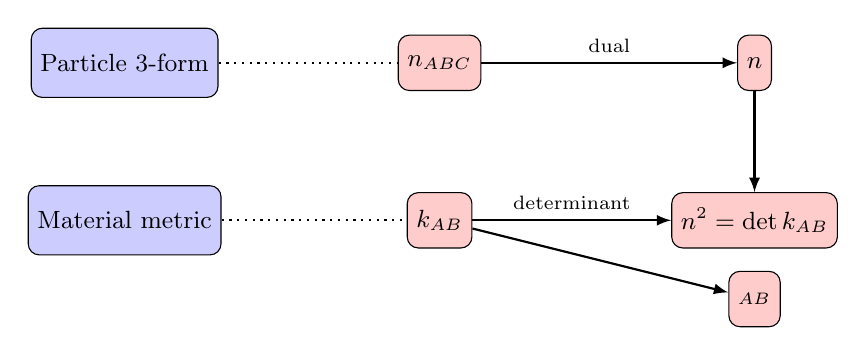
\begin{tikzpicture}[node distance = 2cm, auto]
    % Place nodes
    \node [block2] (form) {{\small Particle 3-form}};
    \node [block, right of=form, node distance=4cm] (form_1) {\small $n_{ABC}$};   
    \node [block, right of=form_1, node distance=4cm] (form_2) {\small $n$};        
    \node [block2, below of=form] (metric) {{\small Material metric}};        
    \node [block, right of=metric, node distance=4cm] (metric_1) {\small $k_{AB}$};     
    \draw [line1] (metric) -- (metric_1);
    \node [block, right of=metric_1, node distance=4cm] (metric_2) {\small $n^2 = \det k_{AB}$};        
    \node [block, below of=metric_2, node distance=1cm] (metric_3) {\small $\unimod_{AB}$};            
    % Draw edges
    \draw [line1] (form) -- (form_1);
    \draw [line] (form_1) -- node{\scriptsize dual}(form_2);
        \draw [line] (metric_1) -- node{\scriptsize determinant}(metric_2);
    \draw [line] (form_2) -- (metric_2);    
       \draw [line] (metric_1) -- (metric_3);        
\end{tikzpicture}
\caption{Explanation of the link between geometrical objects in  the particle 3-form and material-metric formulations of elasticity theory. In the ``particle 3-form'' formulation, the only peice of information about the geometrical structure of the material manifold that is actually used is $n$, the dual of the particle 3-form. In the ``material metric'' formulation, one posits a metric on the material manifold which has more pieces of information which are used: its determinant, $n$, and quantites $\eta_{AB}$ which keep track of the shear-like parts of $k_{AB}$. The point is that the material metric construction keeps track of more information about the material manifold than the particle 3-form construction. In this way the former is more general than the latter.}\label{fig:obj_links}
\end{centering}
\end{figure}
 